\documentclass{article}
\usepackage[hidelinks]{hyperref}
\usepackage{graphicx}
\usepackage{amsfonts}
\usepackage{amsmath}
\usepackage{enumitem}
\usepackage{polski}
\usepackage[utf8]{inputenc}
\usepackage{indentfirst}
\usepackage{float}
\title{Dokumentacja projektu dotyczącego optymalnego układania klocków na planszy}
\author{Abdelkarim Ahmed, Cacko Agata, Hernik Aleksandra}
\begin{document}
\maketitle
\section{Opis projektu}

\clearpage
\section{Opis algorytmu}
Wykorzystany algorytm jest algorytmem zachłannym z określoną parametrem liczbą nawrotów $k$. W każdym kroku algorytmu uruchamiane jest $k'$, gdzie $1 \le k' \le k$ (w sekcji wielowątkowość znajduje się wyjaśnienie, od czego jest uzależniona ich dokładna liczba). Każdemu wątkowi odpowiada jeden z $k$ najlepszych wyników uzyskanych w poprzednim kroku, gdzie najlepszy wynik to taki, dla którego wartość funkcji kosztu jest jak najmniejsza -- każdy z nich dla swoich danych wejściowych znajduje $k$ najlepszych rozwiązań. Znalezienie rozwiązań polega na sprawdzeniu dla każdego klocka każdego jego rotacji -- najpierw wybierana jest jego pozycja, a następnie liczony koszt całej planszy. $k$ rozwiązań takich, że funkcja kosztu obliczona na planszy z położonym danym klockiem w danej rotacji jest najmniejsza, to rozwiązanie dla danego wątku. Następnie, spośród ułożeń otrzymanych przez wszystkie wątki ($1 \le k' \le k$, zatem otrzymywane jest od $k$ do $k^2$ ułożeń) wybierane jest $k$ najlepszych. Ogólny schemat działania algorytmu podsumowuje poniższy diagram:
\begin{figure}[H]
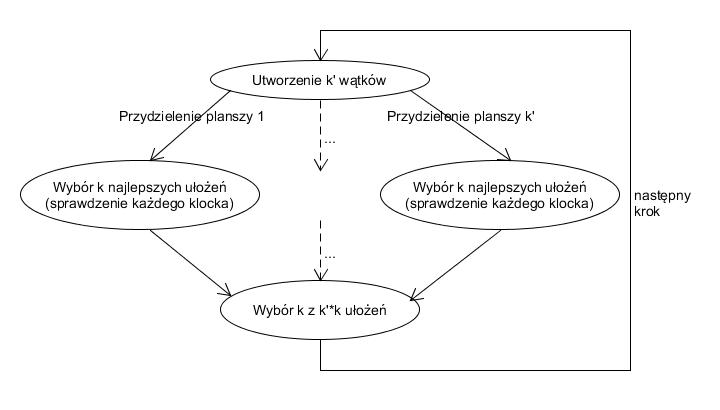
\includegraphics[width=\textwidth]{schemat_algorytmu.png}
\caption{Ogólny schemat działania algorytmu}
\end{figure}
\subsection{Wybór pozycji dla klocka}
\subsection{Funkcje kosztu planszy}
Aplikacja umożliwia wybór funkcji kosztu, która jest wykorzystywana w trakcie działania algorytmu. Wszystkie funkcje kosztu przyjmują jako parametr planszę i zwracają liczbę całkowitą -- im niższy wynik, tym lepsze rozwiązanie. Dostępne są następujące funkcje:
\begin{itemize}
\item \textit{Najmniej dziur} -- wynik to liczba dziur, przy czym dziura jest definiowana jako każde puste pole takie, że co najmniej jedno pole znajdujące się wyżej jest zajęte.
\item \textit{Najmniejsza wysokość} -- wynik to wysokość najwyższej kolumny.
\item \textit{Największa przyległość} -- wynik to wartość przeciwna do sumy długości fragmentów krawędzi klocków, które przylegają do innych klocków lub ścian.
\item \textit{Najładniejsze puste pola} -- funkcja eksperymentalna, której wynik to iloraz liczby dziur, definiowanych tak jak w funkcji \textit{Najmniej dziur}, i liczby zapełnionych pól.
\item \textit{Najmniej dziur ze średnią} -- wprowadzona pod koniec testów usprawniona wersja funkcji minimalizującej liczbę dziur. Usprawnienie polega na tym, że jako dziury liczone są również puste pola znajdujące się poniżej zaokrąglonej średniej z wysokości kolumn, co zapobiega tworzeniu ``kominów''.
\end{itemize}
\subsection{Wielowątkowość}
W celu przyspieszenia działania algorytmu, do wykonywania niezależnych od siebie obliczeń wykorzystywany jest mechanizm wątków. W tym przypadku takimi obliczeniami jest szukanie $k$ najlepszych rozwiązań dla danej planszy. W każdym kroku tworzone jest $k'$ wątków, gdzie $1 \le k' \le k$, a w większości przypadków $k'=k$. 

Pierwszym ze szczególnych przypadków jest pierwszy krok - ponieważ jest tylko jedno wcześniejsze ułożenie (pusta plansza), uruchamiany jest tylko jeden wątek -- gdyby było uruchomione k wątków, każdy z nich znalazł by te same rozwiązania i w efekcie algorytm wybrałby najlepsze rozwiązanie z każdego wątku -- czyli wynikiem pierwszego kroku byłoby k identycznych ułożeń. Dzięki uruchomieniu tylko jednego wątku, znajdowane jest k różnych ułożeń, a ponadto, szczególnie dla dużych k, wykonuje się on szybciej. 

Drugi przypadek jest efektem dodatkowego usprawnienia algorytmu, który ma na celu eliminowanie identycznych rozwiązań, w celu sprawdzenia jak największej liczby możliwości. Polega ono na tym, że po każdym kroku sprawdzana jest unikalność rozwiązań -- sprawdzany jest najpierw ostatni położony klocek (współrzędne, w których został położony, obrót i identyfikator). Jeśli wykryty zostanie jakikolwiek konflikt, dokonywane jest porównanie plansz wynikowych. W przypadku, gdy plansze również są identyczne, pozostawiane jest tylko jedno z tych rozwiązań -- bo identyczne plansze dają identyczne rozwiązania, więc dopóki jakieś rozwiązanie pochodzące z tej planszy byłoby jednym z $k$ najlepszych istniejących, dwa wątki wykonywałyby dokładnie te same operacje. W ten sposób do następnego kroku może trafić zredukowana liczba plansz wejściowych, ale krok później, o ile znowu nie występowały powtórzenia, algorytm stabilizuje liczbę wątków na $k$. Koszt takiego rozwiązania jest niewielki -- porównanie wstępne jest realizowane w czasie stałym (liczba porównań jest rzędu $k^2$, gdzie $k$ to stała, a porównanie ułożenia klocka to cztery porównania liczb całkowitych), więc jeśli problem nie wystąpi, algorytm nie działa zauważalnie wolniej. Liczba sytuacji, w których trzeba wykonać dodatkowe sprawdzenie, powinna być bardzo niewielka, a eliminacja identycznych rozwiązań eliminuje jednakowe obliczenia, które mogłyby ciągnąć się nawet do samego końca -- efektywnie algorytm działałby od pewnego momentu tak, jakby wartość $k$ została zmniejszona.

Po zwróceniu przez każdy z $k$ wątków listy $k$ najlepszych rozwiązań trzeba wybrać k najlepszych rozwiązań z otrzymanych $k^2$.  
Wynikowe elementy są wybierane przez k-krotny wybór największego elementu z list.
Korzystamy tu z faktu, że zwrócone listy są posortowane po wartości funkcji kosztu.
Dzięki temu wystarczy sprawdzić tylko najmniejszy niewykorzystany element z każdej listy (w czasie $k$), zamiast przeglądać wszystkie elementy wszystkich list (w czasie $k^2$).
\subsection{Struktura danych}

\clearpage
\section{Wydajność}
Testy wydajnościowe były wykonywane na komputerze z dość starym procesorem AMD Phenom II X4 965 BE, który jest znacznie wolniejszy od procesora Intel Core i7 2600K w komputerach laboratoryjnych, a ponadto nie posiada funkcjonalności hyperthreading, która znacząco zwiększa wydajność aplikacji wielowątkowych. Mimo tego, wykonanie algorytmu nawet dla dużych zestawów danych trwało co najwyżej kilkadziesiąt sekund.

Pierwszy przeprowadzony test polegał na porównaniu wydajności funkcji kosztu dla zestawu 200, 400 i 600 klocków dla parametru $k = 4$. Rezultaty znajdują się na wykresie poniżej:
\begin{figure}[H]
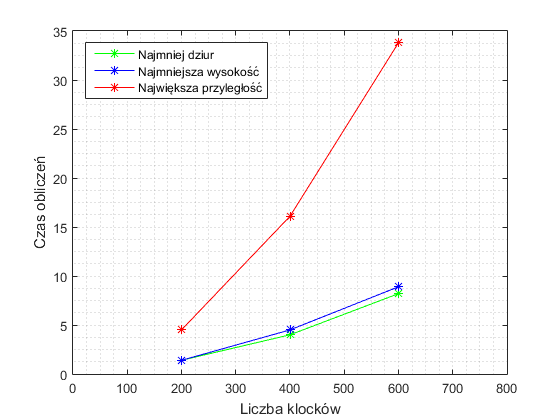
\includegraphics[width=\textwidth]{wydajnosc_porownanie_funkcji.png}
\caption{Porównanie wydajności funkcji kosztu}
\end{figure}
Jak widać, funkcja maksymalizująca przyległość jest znacznie wolniejsza od dwóch pozostałych, których wydajność jest prawie identyczna. Był to spodziewany rezultat, ponieważ ta funkcja dla każdego pola w tablicy musi dokonać pięciu sprawdzeń (czy fragment klocka dotyka lewej ściany, prawej ściany, podłogi, fragmentu innego klocka z prawej strony i fragmentu innego klocka na górze), w przeciwieństwie do pozostałych funkcji, które dokonują tylko jednego sprawdzenia. Spodziewanym rezultatem był również duży wpływ funkcji kosztu na czas działania całego algorytmu -- funkcja kosztu jest wywoływana w każdym kroku przez każdy wątek tyle razy, ile jest możliwych do uzyskania przez ten algorytm ułożeń.

Drugi test sprawdza wpływ zmiany parametru $k$ na wydajność algorytmu. Sprawdzane były wartości 1, 2, 3, 4, 6, 8 i 10 dla funkcji \textit{Najmniej dziur} oraz zestawu 200, 400 i 600 klocków. Poniższy wykres obrazuje wyniki:
\begin{figure}[H]
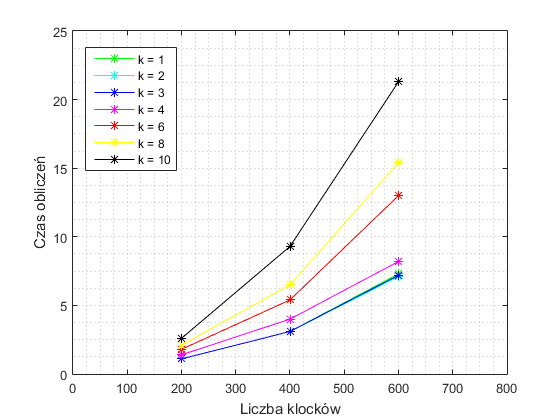
\includegraphics[width=\textwidth]{porownanie_k.png}
\caption{Porównanie wydajności dla różnych wartości parametru}
\end{figure}
Również w tym teście wyniki nie zaskakują. Wyniki dla wartości $k$ równych 1, 2 i 3 są identyczne, ponieważ procesor, na którym wykonywane były testy, ma cztery rdzenie -- jeden z nich zawsze jest częściowo wykorzystywany przez inne działające aplikacje (w tym system operacyjny), a także interfejs użytkownika. Pozostałe trzy w całości mogły poświęcić się liczeniu algorytmu. Stąd też bardzo niewielki skok przy zmianie $k$ z 3 na 4. Dalszy wzrost wynika przede wszystkim z braku możliwości rzeczywistego jednoczesnego obliczania wszystkich wątków i częściowo z narzutu wynikającego z ich tworzenia.

Zauważonym problemem jest znaczne spowolnienie działania interfejsu przy dużej liczbie klocków -- wynika to z ręcznego rysowania każdego fragmentu krawędzi klocka oddzielnie, co przypuszczalnie sprawia, że do karty graficznej przesyłane jest dużo małych poleceń rysowania, zamiast jednego większego. Dzięki temu jednak wizualizacja jest znacznie czytelniejsza niż w przypadku aplikacji, w których klocki oddzielane są jedynie kolorem. 
\clearpage


\subsubsection{Klasa Algorithm}
Główną klasą naszego programu jest klasa Algorithm. Przechowuje ona wszystkie dane dotyczące algorytmu i wykonuje kolejne kroki. 

\subsubsection{Klasa Board}
Klasa Board odpowiada za przechowywanie zawartości studni (jest to tablica intów).

Ważne metody:
\begin{itemize}
\item \textbf{AddBlock} -- sprawdza możliwość dodania klocka na planszę (czy miejsce, w które chcemy położyć klocek, jest wolne), po czym zmniejsza o jeden liczbę dostępnych klocków tego typu i wpisuje klocek w odpowiednie miejsce na planszy.
\item DeleteBlock(BlockType block) -- usuwa klocek ze studni. Nie ma żadnych mechanizmów weryfikacji, czy faktycznie klocek leżący w danym miejscu na planszy jest tym samym klockiem co ten, którego chcemy z planszy usunąć. Taka weryfikacja jednak nie jest potrzebna, ponieważ stosujemy algorytm zachłanny, zatem usuwanie klocków wcześniej położonych nie jest w ogóle potrzebne. W przypadku naszego programu stosowane jest to jednak przy wyborze najlepszego miejsca na kolejny klocek, gdy dodajemy i usuwamy kolejne klocki w różnych miejscach na tymczasowej planszy.
\item ChooseBlocks
\end{itemize}





\section{Testy}
\subsection{Zestaw 100 klocków 4x3, 5x3, 5x4, 6x4 o polu co najwyżej 8}
Na tym standardowym zestawie klocków zostanie dokonana dokładna analiza własności naszego algorytmu z uwzględnieniem różnej liczby rozgałęzień, szerokości studni i wszystkich udostępnionych funkcji kosztu.

\subsubsection{Szerokość studni: 5}
\begin{enumerate}
\item Funkcja minimalizująca dziury

Gęstość dla $k=3$: 71

Najlepsza gęstość dla $k=5$: 71

Dla podanych parametrów można zauważyć ciekawe zachowanie. 
Wbrew oczekiwaniom zwiększaniu liczby rozgałęzień nie towarzyszy poprawa wyników. 
Najlepszy wynik wystąpił dla $k=5$ i $k=10$ przy znacznie niższych wartościach dla wartości pomiędzy. W
ynika to ze specyfiki zastosowanego algorytmu, będącego algorytmem zachłannym. 
Na przykład dla $k=4$ w trakcie obliczeń mogło pojawić się ułożenie, które w danym momencie wydawało się bardziej obiecujące, niż wszystkie ułożenia dla $k=3$, jednak ostatecznie okazało się mniej korzystne.
Podobny efekt można zaobserwować dla pozostałych funkcji.

\begin{figure}[H]
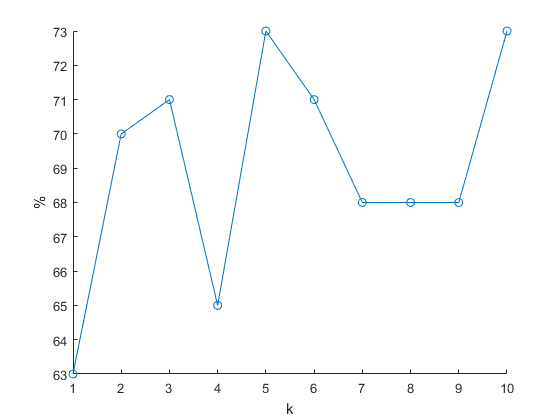
\includegraphics[width=\textwidth]{k_plot.png}
\caption{Wykres gęstości od liczby rozgałęzień}
\end{figure}

\item Funkcja minimalizująca wysokość

Gęstość dla $k=3$: 71

Najlepsza gęstość dla $k=10$: 75

Funkcja wysokości, nie najlepiej sprawdzająca się w większości przypadków, przy wąskiej studni radzi sobie porównywalnie z pozostałymi.

\item Funkcja maksymalizująca przyleganie

Gęstość dla $k=3$: 70

Najlepsza gęstość dla $k=7$: 76

Jest to najlepsza funkcja dla tego przypadku - dobry rezultat udało się osiągnąć przy stosunkowo małej wartości k.
\end{enumerate}
\subsubsection{Szerokość studni: 20}
Szerokość 20 jest najlepsza do porównania funkcji kosztu, a także zaobserwowania ich szczególnych cech.
Pozwala na większą swobodę ułożenia klocków niż szerokość 5, a jednocześnie wynikowa wysokość jest na tyle duża, że nierówności na górze nie mają istotnego wpływu na gęstość.
\begin{enumerate}
\item Funkcja minimalizująca dziury

Gęstość dla $k=3$: 75

Najlepsza gęstość dla $k=9$: 80

Na rysunku można zaobserwować pewną wadę tej funkcji - pozwala na tworzenie głębokich, wąskich dziur (jak na górze po lewej). 
Wynika to z tego, że takie zjawisko nie jest traktowane przez funkcję jako dziura.
Z kolei zakrycie takiej dziury klockiem znacząco zwiększa liczbę dziur, więc algorytm pozwoli na to tylko w ostateczności.

\begin{figure}[H]
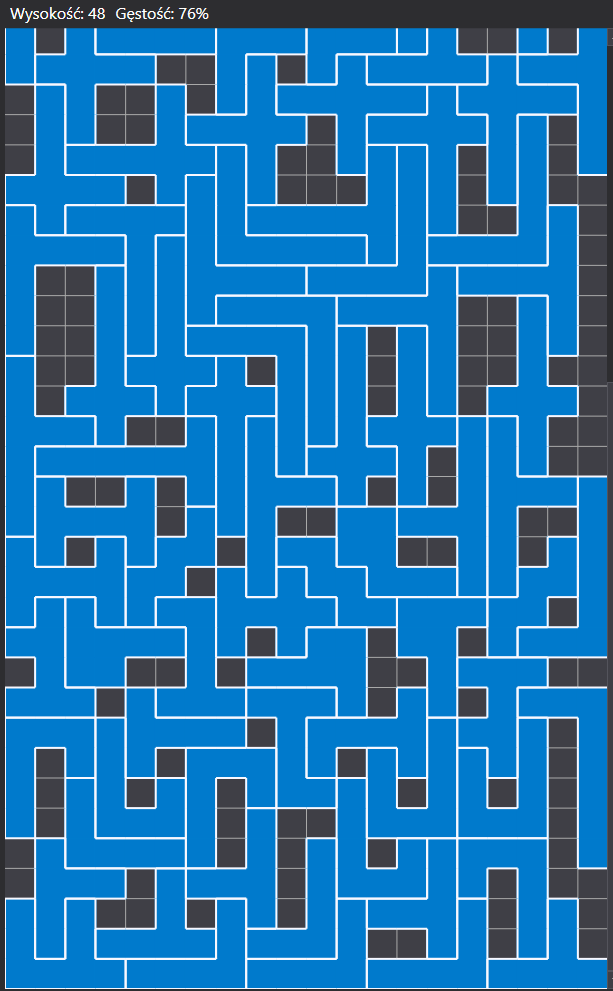
\includegraphics[width=\textwidth]{dziury.PNG}
\caption{Ułożenie klocków dla funkcji dziur}
\end{figure}

\item Funkcja minimalizująca wysokość

Gęstość dla $k=3$: 72

Najlepsza gęstość dla $k=10$: 76

W przypadku funkcji wysokości można zauważyć ciekawy wizualny efekt - klocki wydają się być położone maksymalnie poziomo.
Wynika to z faktu, że takie położenie minimalizuje wysokość w danym ruchu - nie ma znaczenia, że za kilka ruchów może się okazać niekorzystne.

\begin{figure}[H]
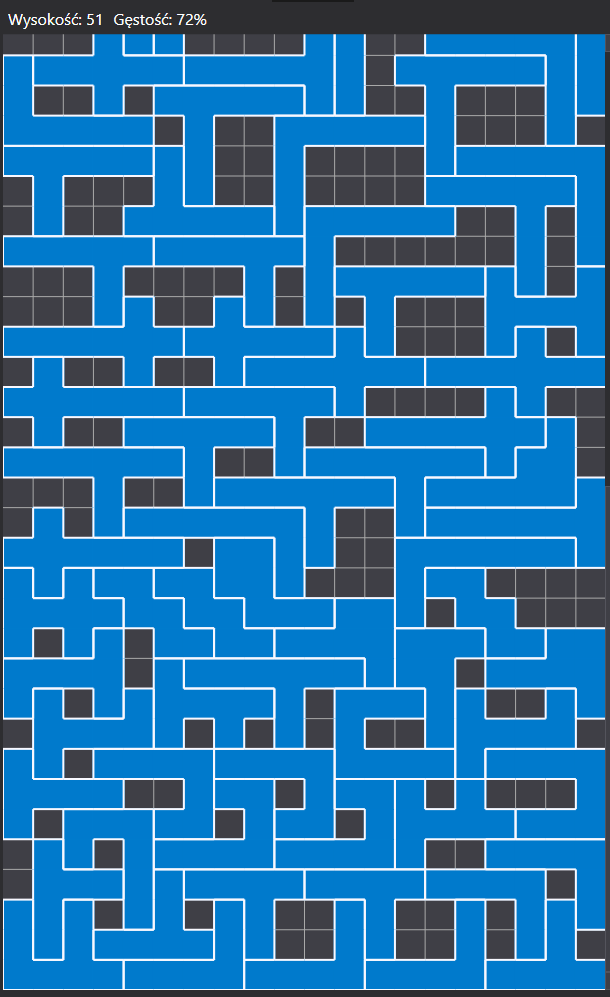
\includegraphics[width=\textwidth]{wysokosc.PNG}
\caption{Ułożenie klocków dla funkcji wysokości}
\end{figure}

\item Funkcja maksymalizująca przyleganie

Gęstość dla $k=3$: 76

Najlepsza gęstość dla $k=8$: 83

Funkcja przylegania sprawdziła się w tym przypadku najlepiej.

\begin{figure}[H]
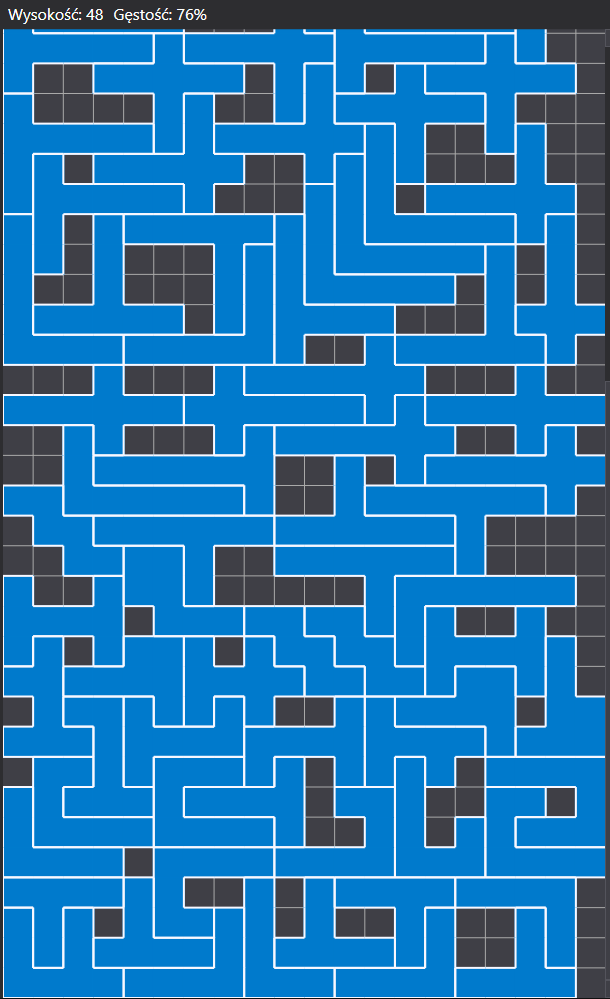
\includegraphics[width=\textwidth]{przyleglosc.PNG}
\caption{Ułożenie klocków dla funkcji przyległości}
\end{figure}

\end{enumerate}
\subsubsection{Szerokość studni: 80}
\begin{enumerate}

\item Funkcja minimalizująca dziury

Gęstość dla $k=3$: 66

Najlepsza gęstość dla $k=5$: 71

\begin{figure}[H]
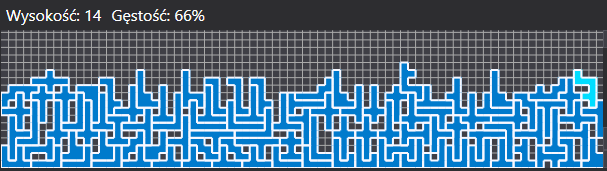
\includegraphics[width=\textwidth]{szeroka_plansza.PNG}
\caption{Ułożenie klocków dla funkcji przyległości}
\end{figure}

\item Funkcja minimalizująca wysokość

Gęstość dla $k=3$: 66

Najlepsza gęstość dla $k=9$: 66

\item Funkcja maksymalizująca przyleganie

Gęstość dla $k=3$: 66

Najlepsza gęstość dla $k=5$: 71

\end{enumerate}
\textbf{Wnioski}

W tym teście najlepsza okazała się funkcja przylegania, jednak niewiele tylko wyprzedziła funkcję dziur.

Warto zauważyć, że algorytm daje najlepsze wyniki dla średniej szerokości studni, co zgadza się z intuicją.
W przypadku małej szerokości, porównywalnej z szerokością niektórych klocków trudno jest osiągnąć dobre zapełnienie dziur - w niektórych momentach konieczne jest praktycznie układanie klocków jeden na drugim.
Z kolei przy szerokiej studni na wynik niekorzystnie wpływają górne mało zapełnione wiersze.

\subsection{Zestaw klocków prostokątnych}
W tym zadaniu największym problemem jest górna część planszy - do pewnego momentu klocki są układane prawie bez tworzenia dziur. Jednak dla dużego k jest znajdowane rozwiązanie, w którym nie pojawia się ten problem.
\begin{enumerate}

\item Funkcja minimalizująca dziury

Gęstość dla $k=3$: 88

Najlepsza gęstość dla $k=5$: 91

Funkcja ta wypadła słabo ze względu na powstałą głęboką, wąską dziurę.
\begin{figure}[H]
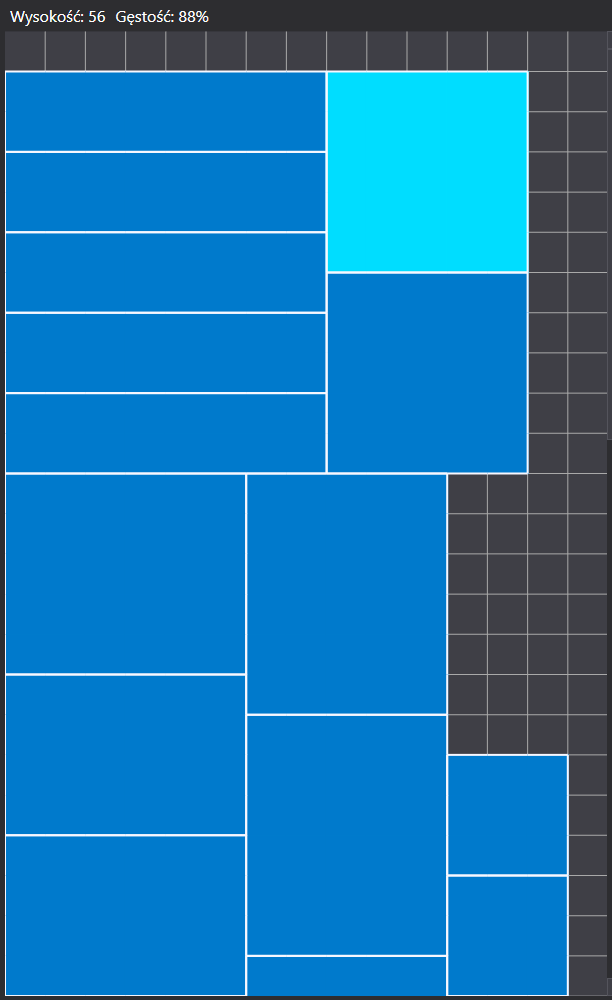
\includegraphics[width=\textwidth]{prostokaty_dziury.PNG}
\caption{Górna część wyniku dla funkcji dziur}
\end{figure}


\item Funkcja minimalizująca wysokość

Gęstość dla $k=3$: 89

Najlepsza gęstość dla $k=4$: 91

Problemem w tej funkcji okazał się fakt, że na końcu nie zostały żadne wąskie klocki - wcześniej zostały wykorzystane, bo kładzenie ich poziomo pozwalało na chwilową minimalizację wysokości.
\begin{figure}[H]
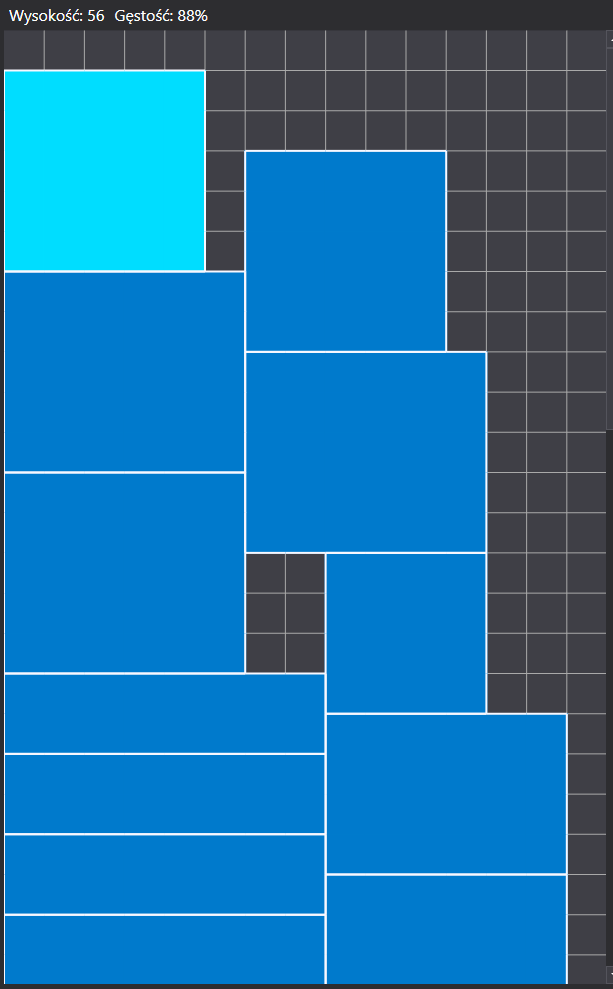
\includegraphics[width=\textwidth]{prostokaty_wysokosc.PNG}
\caption{Górna część wyniku dla funkcji wysokości}
\end{figure}

\item Funkcja maksymalizująca przyleganie

Gęstość dla $k=3$: 91

Najlepsza gęstość dla $k=5$: 96

Rozwiązanie dla $k=5$ wydaje się być bardzo dobre - być może najlepsze, jakie można uzyskać dla tego zadania.
\begin{figure}[H]
\hspace*{3.5cm}
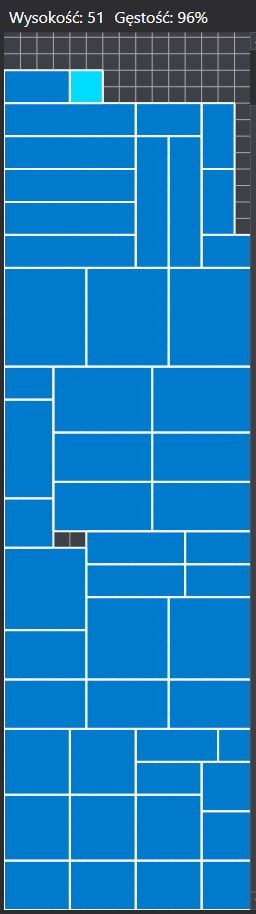
\includegraphics[width=5.3cm]{prostokaty.PNG}
\caption{Najlepsze rozwiązanie dla prostokątów}
\end{figure}

\end{enumerate}
\subsection{Zestaw klocków o różnorodnych rozmiarach i kształtach (grupy Marcina Rudnika)}
Nasz algorytm dobrze radzi sobie z tym testem. 
Wynika to z kilku cech naszego rozwiązania.
Po pierwsze umożliwiamy wstawianie klocków w powstałe wcześniej dziury - na rysunku poniżej można zaobserwować kilka klocków, które idealnie gdzieś się wpasowały.
Ponadto funkcja przyległości (która okazała się najlepsza) faworyzuje duże klocki, co w tym wypadku jest korzystne - lepiej potem wypełnić powstałe dziury, niż najpierw szczelnie wypełnić dół planszy małymi klockami.
\begin{enumerate}

\item Funkcja minimalizująca dziury

Gęstość dla $k=3$: 73

Najlepsza gęstość dla $k=4$: 75

\item Funkcja minimalizująca wysokość

Gęstość dla $k=3$: 69

Najlepsza gęstość dla $k=69$: 73

\item Funkcja maksymalizująca przyleganie

Gęstość dla $k=3$: 78

Najlepsza gęstość dla $k=8$: 81

\begin{figure}[H]
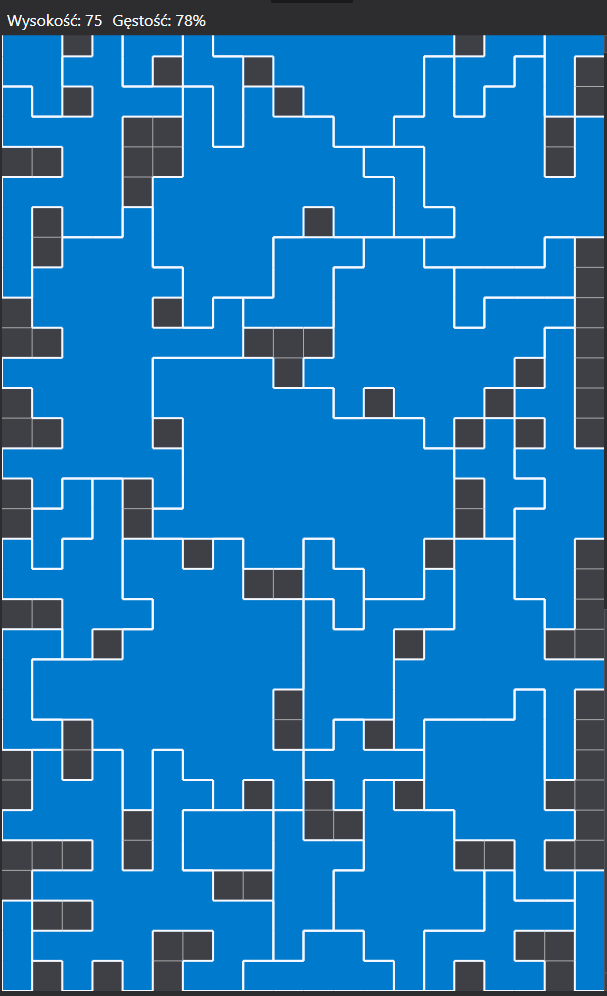
\includegraphics[width=\textwidth]{duze_klocki.PNG}
\caption{Ułożenie dużych klocków dla funkcji przyległości}
\end{figure}

\end{enumerate}


\subsection{Zestaw 120 klocków 5x4 o polu 9, z szerokością studni 10, grupy Mirona Marczuka}
\begin{enumerate}

\item Funkcja minimalizująca dziury

Gęstość dla $k=3$: 65

Najlepsza gęstość dla $k=7$: 68

\item Ulepszona funkcja minimalizująca dziury

Gęstość dla $k=3$: 73

Najlepsza gęstość dla $k=10$: 80

\item Funkcja minimalizująca wysokość

Gęstość dla $k=3$: 72

Najlepsza gęstość dla $k=8$: 78

\item Funkcja maksymalizująca przyleganie

Gęstość dla $k=3$: 68

Najlepsza gęstość dla $k=10$: 78

\end{enumerate}
\textbf{Wnioski}

W tym teście z wcześniej wykorzystywanych funkcji zdecydowanie odstawała jedynie funkcja minimalizująca dziury. Powód jest taki sam jak we wcześniej omawianym przykładzie -- algorytm pozostawia pustą kolumnę, co bardzo negatywnie wpływa na wynik. Z kolei wynik algorytmu minimalizującego wysokość jest bardzo dobry, bo wszystkie klocki mają bardzo zbliżoną wysokość i szerokość, tak więc algorytm nie próbuje po prostu położyć poziomo na spodzie wszystkich podłużnych klocków.

Testowo została wprowadzona tu omówiona wcześniej ulepszona wersja funkcji minimalizującej dziury, która okazała się w tym przypadku być najlepszą ze wszystkich, ponieważ usprawnienie rzeczywiście wyeliminowało tworzenie się pustej kolumny.

\subsection{Zestaw 124 klocków 5x4 i 6x4 o polu 9, z szerokością studni 80, grupy Anny Bekas}
Głównym problemem tego zestawu jest nieproporcjonalnie szeroka studnia w porównaniu do liczby i wielkości klocków.
\begin{enumerate}

\item Funkcja minimalizująca dziury

Gęstość dla $k=3$: 63

Najlepsza gęstość dla $k=5$: 66

\item Ulepszona funkcja minimalizująca dziury

Gęstość dla $k=3$: 66

Najlepsza gęstość dla $k=3$: 66

\item Funkcja minimalizująca wysokość

Gęstość dla $k=3$: 52

Najlepsza gęstość dla $k=4$: 66

\item Funkcja maksymalizująca przyleganie

Gęstość dla $k=3$: 63

Najlepsza gęstość dla $k=10$: 73

\end{enumerate}
\textbf{Wnioski}

Najlepsza okazała się funkcja maksymalizująca przyleganie. Dla funkcji minimalizującej dziury zwiększanie parametru $k$ nie poprawiało rezultatów, ze względu na bardzo szeroką studnię w stosunku do liczby klocków -- przez cały pierwszy wiersz w praktyce nie pojawiały się żadne dziury. Jej usprawniona wersja osiągnęła taki sam maksymalny wynik, ale dla trochę niższej wartości parametru $k$ -- tutaj powstawanie kolumny nie było znaczącym problemem.
Ciekawe zachowanie funkcji minimalizującej wysokość (duży przeskok z $k=3$ do $k=4$, a następnie brak poprawy) jest bardzo łatwy do wytłumaczenia -- zwiększenie $k$ ``zmusiło" algorytm do rozważenia znacznie lepszej rotacji, która na początku nie ma znaczenia, ale później decydowała o całym ułożeniu. Opisana różnica jest przedstawiona na poniższym rysunku: 
\begin{figure}[H]
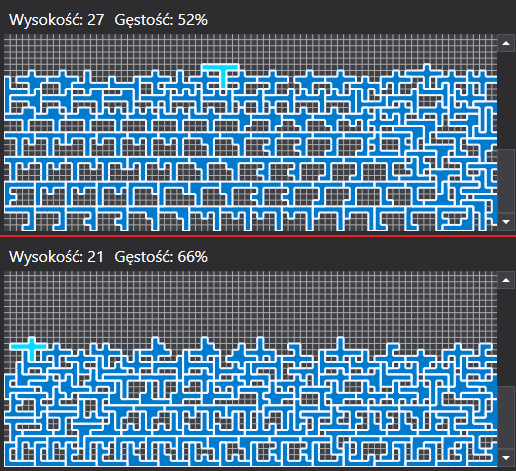
\includegraphics[width=\textwidth]{wysokosc_bekas.PNG}
\caption{Ułożenie klocków dla funkcji wysokości}
\end{figure}


%\subsection{zestaw drugi...}


\section{Wnioski} %z testów
\end{document}